% =====================================================================
%  Slide bảo vệ khóa luận -- HQMoSS-Net
%  Biên dịch: xelatex slides.tex  (chạy 2 lần để footer x/tổng đúng)
%  Font: Segoe UI (hỗ trợ tiếng Việt đầy đủ). Hình tái sử dụng từ figures/.
% =====================================================================
\documentclass[aspectratio=169,11pt]{beamer}

\usepackage{fontspec}
\usepackage{amsmath,amssymb}
\usepackage{graphicx}
\usepackage{booktabs}
\usepackage{array}
\usepackage{colortbl}
\usepackage{tikz}
\usepackage{xcolor}
\usepackage{appendixnumberbeamer} % giữ số trang phần chính, phụ lục đánh số riêng

% ---------- Font (XeLaTeX + tiếng Việt) ----------
\setsansfont{Segoe UI}
\setmainfont{Segoe UI}

% ---------- Bảng màu (logo KHTN -- xanh navy) ----------
\definecolor{hcmusblue}{RGB}{18,59,110}
\definecolor{hcmusmid}{RGB}{37,95,160}
\definecolor{hcmusaccent}{RGB}{198,146,42}
\definecolor{softgray}{RGB}{240,242,245}

% ---------- Theme tối giản, học thuật ----------
\usetheme{default}
\useinnertheme{circles}
\setbeamertemplate{navigation symbols}{}
\setbeamercolor{structure}{fg=hcmusblue}
\setbeamercolor{frametitle}{fg=hcmusblue}
\setbeamercolor{title}{fg=hcmusblue}
\setbeamercolor{block title}{fg=white,bg=hcmusmid}
\setbeamercolor{block body}{bg=softgray}
\setbeamercolor{alerted text}{fg=hcmusaccent}
\setbeamercolor{itemize item}{fg=hcmusblue}
\setbeamercolor{itemize subitem}{fg=hcmusmid}
\setbeamerfont{frametitle}{series=\bfseries}
\setbeamerfont{title}{series=\bfseries,size=\LARGE}
\setbeamertemplate{itemize item}{\small\raise0.3ex\hbox{\textbullet}}

% ---------- Thanh tiêu đề khung (nền trắng + chữ navy + gạch + logo) ----------
\setbeamertemplate{frametitle}{%
  \vspace{0.4em}%
  \begin{beamercolorbox}[wd=\paperwidth,leftskip=0.7em,rightskip=0.7em]{frametitle}%
    \begin{minipage}[c]{0.82\paperwidth}%
      \usebeamerfont{frametitle}\insertframetitle%
    \end{minipage}\hfill%
    \raisebox{-0.22em}{
\includegraphics[height=0.82cm]{logo1.png}}%
  \end{beamercolorbox}%
  \vskip1pt{\color{hcmusblue}\hrule height 1pt}%
}

% ---------- Footer: SV | đề tài | trang/tổng ----------
\setbeamercolor{fA}{bg=hcmusblue,fg=white}
\setbeamercolor{fB}{bg=hcmusmid,fg=white}
\setbeamercolor{fC}{bg=hcmusblue,fg=white}
\setbeamertemplate{footline}{%
  \leavevmode%
  \hbox{%
    \begin{beamercolorbox}[wd=.30\paperwidth,ht=2.6ex,dp=1.1ex,leftskip=1em]{fA}%
      \usebeamerfont{footline}N.\,S.\,Trực \textperiodcentered\ P.\,T.\,Vương%
    \end{beamercolorbox}%
    \begin{beamercolorbox}[wd=.55\paperwidth,ht=2.6ex,dp=1.1ex,center]{fB}%
      \usebeamerfont{footline}HQMoSS-Net -- Phân đoạn ảnh y sinh lai lượng tử -- cổ điển%
    \end{beamercolorbox}%
    \begin{beamercolorbox}[wd=.15\paperwidth,ht=2.6ex,dp=1.1ex,rightskip=1em]{fC}%
      \usebeamerfont{footline}\hfill\insertframenumber\,/\,\inserttotalframenumber%
    \end{beamercolorbox}%
  }%
}
\setbeamerfont{footline}{size=\scriptsize}

% Lệnh tắt cho tiêu đề nhấn mạnh
\newcommand{\hl}[1]{\textcolor{hcmusblue}{\textbf{#1}}}
\newcommand{\acc}[1]{\textcolor{hcmusaccent}{\textbf{#1}}}

% =====================================================================
\begin{document}

% ---------- 1. TRANG BÌA ----------
{%
\setbeamertemplate{footline}{}%
\begin{frame}[plain]
  \centering
  \vspace{0.3em}
  
\includegraphics[height=0.20\textheight]{images/logo-khtn.png}\\[0.3em]
  {\small TRƯỜNG ĐẠI HỌC KHOA HỌC TỰ NHIÊN, ĐHQG-HCM\\ KHOA CÔNG NGHỆ THÔNG TIN}\\[0.9em]
  {\color{hcmusblue}\rule{0.85\textwidth}{1pt}}\\[0.7em]
  {\LARGE\bfseries\color{hcmusblue} Xây dựng mạng nơ-ron lai lượng tử -- cổ điển}\\[0.25em]
  {\large\bfseries\color{hcmusblue} dựa trên kiến trúc U-Net cho bài toán phân đoạn ảnh y sinh}\\[0.5em]
  {\color{hcmusblue}\rule{0.85\textwidth}{1pt}}\\[0.9em]
  \begin{columns}[T]
    \column{0.52\textwidth}\centering\small
      \textbf{Sinh viên thực hiện}\\
      Nguyễn Sinh Trực -- 22120395\\
      Phạm Tuấn Vương -- 22120446
    \column{0.48\textwidth}\centering\small
      \textbf{Giảng viên hướng dẫn}\\
      ThS. Phạm Trọng Nghĩa\\
      ThS. Lê Nhựt Nam
  \end{columns}
  \vspace{0.8em}
  {\footnotesize\itshape Khóa luận tốt nghiệp Cử nhân -- TP. Hồ Chí Minh, tháng 07/2026}
\end{frame}
}

% ---------- 2. NỘI DUNG ----------
\begin{frame}{Nội dung trình bày}
  \begin{columns}[T]
    \column{0.5\textwidth}
      \begin{enumerate}
        \item Đặt vấn đề \& động lực
        \item Mục tiêu \& đóng góp
        \item Kiến trúc đề xuất HQMoSS-Net
        \item Thiết lập thực nghiệm
      \end{enumerate}
    \column{0.5\textwidth}
      \begin{enumerate}
        \setcounter{enumi}{4}
        \item Kết quả \& kiểm định thống kê
        \item Phân tích khả giải thích (XAI)
        \item Thảo luận, kết luận \& hướng phát triển
      \end{enumerate}
  \end{columns}
  \vfill
  \begin{block}{Nội dung cốt lõi}
    HQMoSS-Net nhúng khối \hl{hỗn hợp nhánh xử lý lượng tử đa tỷ lệ} (QuantumMoE) và khối \hl{quét chọn lọc} (LSS) vào nút thắt cổ chai của U-Net. Kết quả: hiệu năng vượt trội so với baseline trong khi số tham số nhỏ hơn nhiều lần.
  \end{block}
\end{frame}

% ---------- 3. ĐẶT VẤN ĐỀ ----------
\begin{frame}{Đặt vấn đề: phân đoạn ảnh y sinh}
  \begin{columns}[T]
    \column{0.56\textwidth}
      \begin{itemize}
        \item Phân đoạn ảnh là gán nhãn cho \hl{từng điểm ảnh}, qua đó khoanh vùng tổn thương/cấu trúc một cách chính xác.
        \item Vai trò then chốt trong \hl{chẩn đoán, lập kế hoạch điều trị}.
        \item Phân đoạn thủ công: tốn công, thiếu nhất quán.
        \item Thách thức: \acc{ranh giới mờ}, \acc{đa đối tượng}, \acc{dữ liệu nhỏ} dễ quá khớp.
      \end{itemize}
    \column{0.44\textwidth}
      \centering
      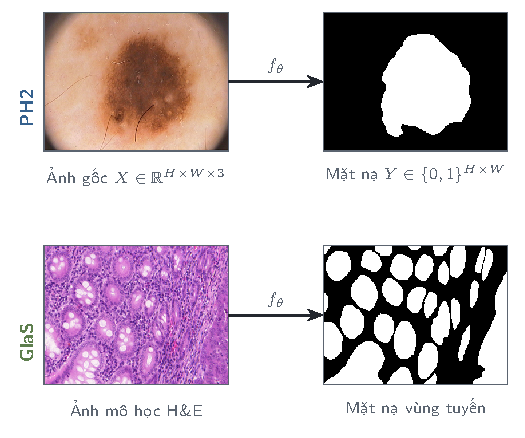
\includegraphics[width=\linewidth,height=0.62\textheight,keepaspectratio]{figures/fig_segmentation_task.pdf}\\
      {\scriptsize Ảnh gốc $\to$ mặt nạ phân đoạn nhị phân.}
  \end{columns}
\end{frame}

% ---------- 4. ĐỘNG LỰC ----------
\begin{frame}{Hạn chế cổ điển \& động lực lượng tử}
  \begin{columns}[T]
    \column{0.5\textwidth}
      \textbf{U-Net và biến thể:}
      \begin{itemize}
        \item Nền tảng chuẩn cho phân đoạn y sinh.
        \item Tuy nhiên, tích chập cổ điển \hl{hạn chế biểu diễn phi tuyến} tại nút thắt cổ chai (độ phân giải thấp nhất).
      \end{itemize}
      \vspace{0.4em}
      \textbf{Học máy lượng tử (QML):}
      \begin{itemize}
        \item Mạch lượng tử tham số hóa (PQC) khai thác không gian Hilbert $2^n$ chiều.
        \item Chồng chất và vướng víu lượng tử cho phép tạo ánh xạ đặc trưng phong phú với số tham số \hl{rất hiệu quả}.
      \end{itemize}
    \column{0.5\textwidth}
      \begin{block}{Khoảng trống nghiên cứu}
        Các mô hình lai lượng tử hiện nay chủ yếu phục vụ bài toán \emph{phân loại}. Việc ứng dụng cho \hl{phân đoạn ảnh y sinh} -- đặc biệt là kết hợp \hl{nhiều nhánh xử lý lượng tử} với khối mô hình hóa chuỗi tại nút thắt cổ chai -- vẫn \acc{còn ít được khảo sát}.
      \end{block}
      \vspace{0.4em}
      \begin{itemize}
        \item Bài toán \hl{giữ cấu trúc không gian} ở đầu ra $\Rightarrow$ khó hơn phân loại.
        \item Cần khối lượng tử \emph{bảo toàn độ phân giải}, chi phí mô phỏng khả thi.
      \end{itemize}
  \end{columns}
\end{frame}

% ---------- 5. NỀN TẢNG LƯỢNG TỬ & QUBIT ----------
\begin{frame}{Nền tảng: điện toán lượng tử \& qubit}
  \begin{columns}[T]
    \column{0.57\textwidth}
      \begin{itemize}
        \item \hl{Qubit} ở trạng thái \hl{chồng chất} (khác bit $0/1$):
      \end{itemize}
      \vspace{-0.3em}
      \[ |\psi\rangle = \alpha|0\rangle + \beta|1\rangle,\quad |\alpha|^2+|\beta|^2=1 \]
      \vspace{-0.5em}
      \begin{itemize}
        \item $n$ qubit $\Rightarrow$ không gian Hilbert \acc{$2^n$ chiều}.
        \item \hl{Vướng víu}: tương quan phi tuyến giữa các qubit.
        \item \hl{Mã hóa biên độ} $+$ \hl{phép đo} $\to$ phân bố xác suất.
      \end{itemize}
    \column{0.43\textwidth}
      \centering
      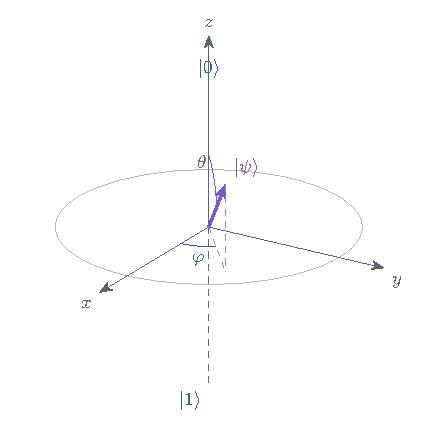
\includegraphics[width=0.74\linewidth,height=0.40\textheight,keepaspectratio]{figures/fig_bloch_sphere.pdf}\\
      {\scriptsize Mặt cầu Bloch: trạng thái một qubit.}
  \end{columns}
  \begin{block}{Ý nghĩa với khóa luận}
    \footnotesize Vài qubit thao tác trên không gian $2^n$ chiều $\Rightarrow$ ánh xạ đặc trưng \hl{giàu biểu diễn, hiệu quả tham số} -- nền tảng cho khối QuantumMoE tại nút thắt cổ chai.
  \end{block}
\end{frame}

% ---------- 6. CỔNG LƯỢNG TỬ ----------
\begin{frame}{Cổng lượng tử -- thành phần cơ bản của mạch}
  \small Mọi phép biến đổi là một cổng \hl{unitary} ($U^\dagger U = I$: thuận nghịch, bảo toàn xác suất). Ba nhóm cổng chính:
  \vspace{0.5em}
  \begin{center}\footnotesize
  \renewcommand{\arraystretch}{1.35}
  \arrayrulecolor{hcmusblue}
  \begin{tabular}{>{\raggedright\arraybackslash}p{2.5cm} >{\raggedright\arraybackslash}p{4.1cm} >{\raggedright\arraybackslash}p{4.9cm}}
    \rowcolor{hcmusblue}
    \textcolor{white}{\textbf{Cổng}} & \textcolor{white}{\textbf{Tác dụng}} & \textcolor{white}{\textbf{Vai trò trong HQMoSS-Net}} \\
    Hadamard $H$ & Tạo \hl{chồng chất} đều: $H|0\rangle=\tfrac{1}{\sqrt2}(|0\rangle{+}|1\rangle)$ & Tầng đầu ansatz -- ``điểm xuất phát'' phong phú \\
    \rowcolor{softgray}
    Cổng quay $R_X,R_Y,R_Z$, $\mathrm{Rot}(\phi,\theta,\omega)$ & \hl{Xoay} điểm Bloch quanh trục $X/Y/Z$ một góc & \acc{Trọng số học được}; trơn theo góc $\Rightarrow$ tính được gradient \\
    CNOT & Đảo qubit đích khi điều khiển $=|1\rangle$ & Tạo \hl{vướng víu}; chuỗi CNOT \emph{khép vòng} nối mọi qubit \\
    \bottomrule
  \end{tabular}
  \arrayrulecolor{black}
  \end{center}
  \vspace{0.3em}
  {\footnotesize\centering Cổng quay $+$ CNOT ghép thành \hl{mạch lượng tử tham số hóa (PQC)} -- lớp học được trích xuất đặc trưng lượng tử.\par}
\end{frame}

% ---------- 7. MỤC TIÊU & ĐÓNG GÓP ----------
\begin{frame}{Mục tiêu \& đóng góp chính}
  \begin{block}{Mục tiêu}
    Thiết kế \& đánh giá kiến trúc lai lượng tử -- cổ điển trên nền U-Net, tăng cường tại nút thắt cổ chai, cho phân đoạn ảnh y sinh.
  \end{block}
  \textbf{Ba đóng góp:}
  \begin{enumerate}
    \item \hl{QuantumMoE đa tỷ lệ}: ba nhánh xử lý lượng tử theo mảnh ảnh nhiều kích thước, điều phối bởi mạng định tuyến + kết nối phần dư.
    \item \hl{Hai khối cổ điển bổ trợ}: khối tích chập đa tỷ lệ \hl{RDMS} mở rộng trường nhìn ở bộ khung, và khối quét chọn lọc \hl{LSS} (lấy cảm hứng từ Mamba) tổng hợp ngữ cảnh toàn cục với chi phí tuyến tính.
    \item \hl{Đánh giá nghiêm ngặt}: 5-fold trên PH2 \& GlaS, kiểm định thống kê (bootstrap CI, meta-analysis) và phân tích khả giải thích Seg-Grad-CAM.
  \end{enumerate}
\end{frame}

% ---------- 6. KIẾN TRÚC TỔNG QUAN ----------
\begin{frame}{Kiến trúc đề xuất HQMoSS-Net}
  \centering
  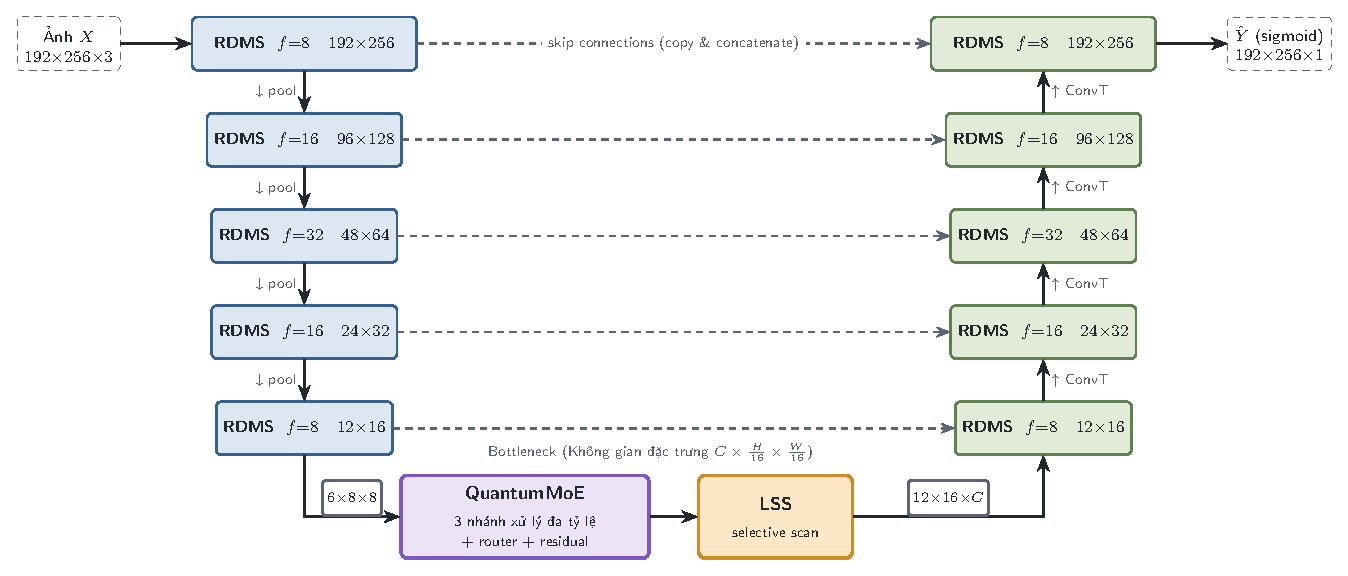
\includegraphics[width=0.96\linewidth,height=0.60\textheight,keepaspectratio]{figures/fig_hqmoss_overview.pdf}\\[0.4em]
  \small Bộ khung U-Net + khối \hl{RDMS} ở encoder/decoder; nút thắt cổ chai nhúng \hl{QuantumMoE} và \hl{LSS}. Ba thành phần này bổ trợ lẫn nhau, chỉ can thiệp tại vùng bottleneck để kiểm soát chi phí tính toán.
\end{frame}

% ---------- 7. HAI KHỐI CỔ ĐIỂN: RDMS & LSS ----------
\begin{frame}{Hai khối cổ điển: RDMS \& LSS}
  \begin{columns}[T]
    \column{0.5\textwidth}
      \centering \textbf{RDMS -- tích chập đa tỷ lệ}\\[0.2em]
      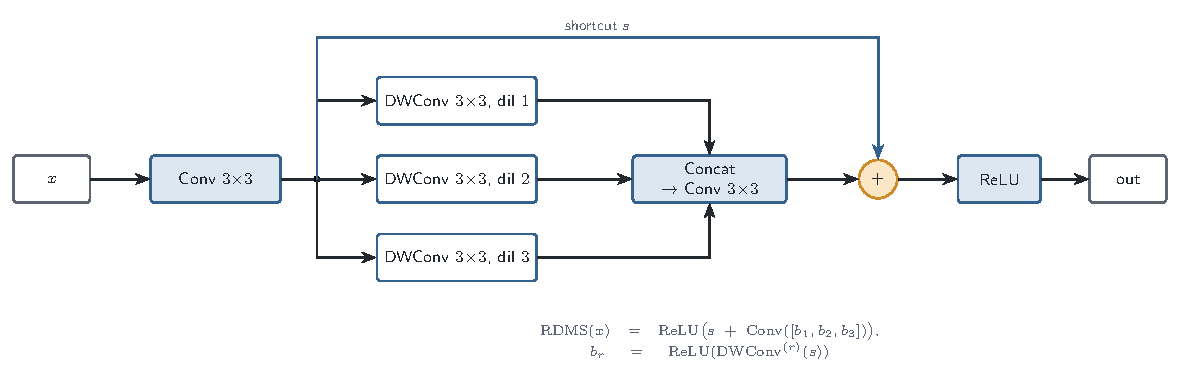
\includegraphics[width=\linewidth,height=0.34\textheight,keepaspectratio]{figures/fig_rdms_block.pdf}\\[0.4em]
      {\scriptsize\raggedright Ba nhánh tích chập tách kênh giãn nở ($r{=}1,2,3$) chạy song song, mở rộng trường nhìn ở nhiều tỷ lệ mà vẫn tiết kiệm tham số; khép lại bằng kết nối phần dư.\par}
    \column{0.5\textwidth}
      \centering \textbf{LSS -- quét chọn lọc (Mamba)}\\[0.2em]
      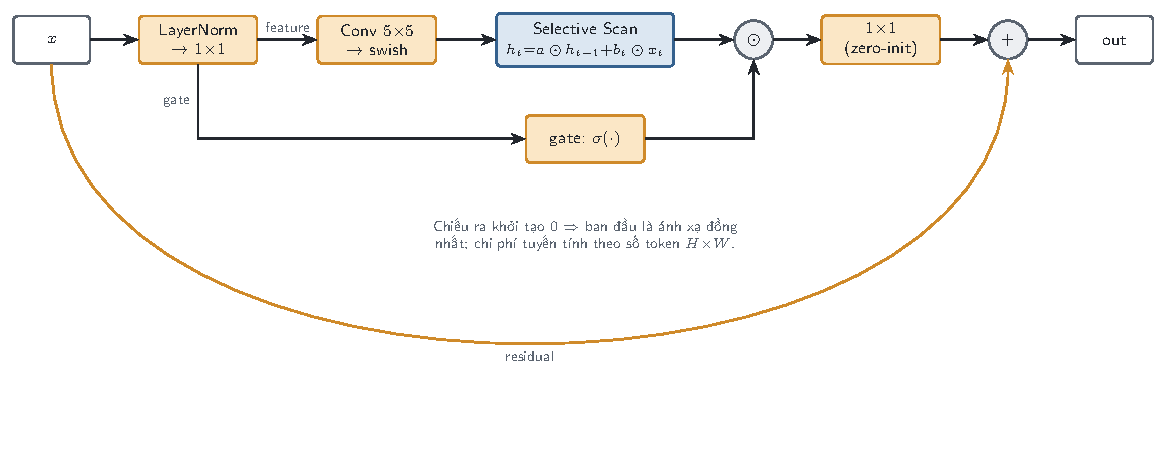
\includegraphics[width=\linewidth,height=0.34\textheight,keepaspectratio]{figures/fig_lss_block.pdf}\\[0.4em]
      {\scriptsize\raggedright Tổng hợp phụ thuộc không gian tầm xa với chi phí \hl{tuyến tính}, bù cho việc các nhánh lượng tử chỉ xử lý từng mảnh ảnh cục bộ.\par}
      {\footnotesize\[ h_t = a\odot h_{t-1} + b_t\odot x_t \]}
  \end{columns}
\end{frame}

% ---------- 8. KHỐI LƯỢNG TỬ: QUANTUMMOE & PQC ----------
\begin{frame}{Khối lượng tử: QuantumMoE \& mạch PQC}
  \begin{columns}[T]
    \column{0.5\textwidth}
      \centering \textbf{QuantumMoE (nút thắt cổ chai)}\\[0.2em]
      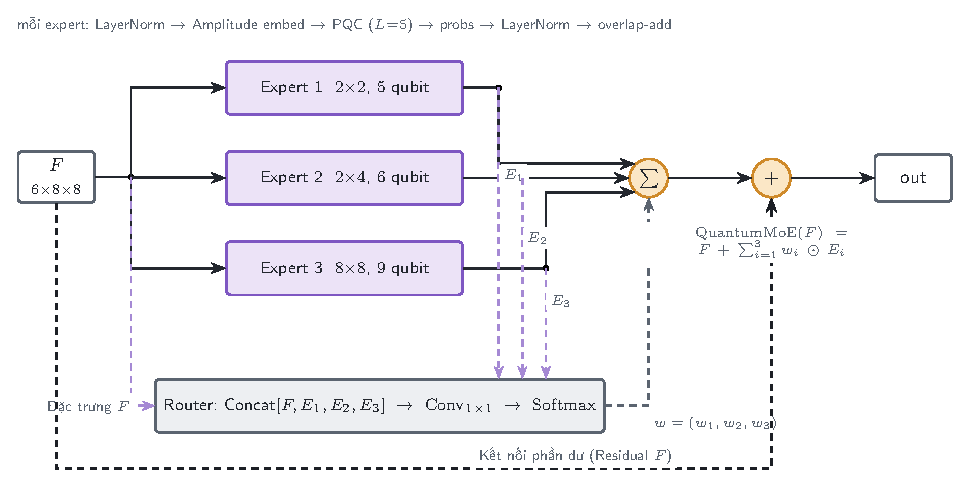
\includegraphics[width=\linewidth,height=0.30\textheight,keepaspectratio]{figures/fig_quantum_moe.pdf}\\[0.35em]
      {\scriptsize\raggedright Ba nhánh xử lý lượng tử đa tỷ lệ; mạng định tuyến trộn đầu ra theo từng điểm ảnh; kết nối phần dư giữ ổn định gradient.\par}
      {\footnotesize\[ \mathrm{QuantumMoE}(F)=F+\textstyle\sum_i w_i\odot E_i \]}
    \column{0.5\textwidth}
      \centering \textbf{Nhánh lượng tử = mạch PQC}\\[0.2em]
      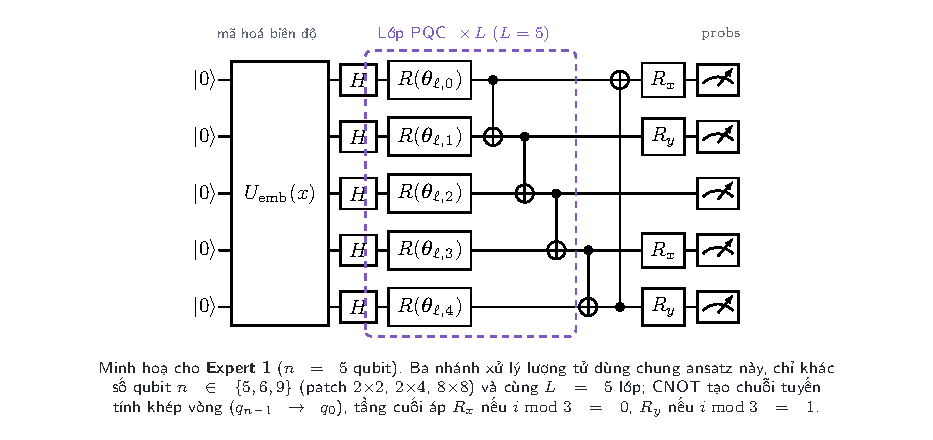
\includegraphics[width=\linewidth,height=0.30\textheight,keepaspectratio]{figures/fig_pqc_main.pdf}\\[0.35em]
      {\scriptsize\raggedright Mã hóa biên độ $\to$ mạch PQC ($L{=}5$) $\to$ đo \texttt{probs}; toàn khối chỉ \acc{320 tham số lượng tử} ($<0.3\%$ mô hình).\par}
      {\footnotesize\[ E(z;\boldsymbol\theta)=\big(|\langle b|U(\boldsymbol\theta)|\psi(z)\rangle|^2\big)_{b} \]}
  \end{columns}
\end{frame}

% ---------- 9. THIẾT LẬP THỰC NGHIỆM ----------
\begin{frame}{Thiết lập thực nghiệm}
  \begin{columns}[T]
    \column{0.46\textwidth}
      \textbf{Dữ liệu} (resize $192\times256$):
      \begin{itemize}
        \item \hl{PH2}: 200 ảnh da liễu, một tổn thương.
        \item \hl{GlaS 2015}: 165 ảnh mô học, đa tuyến -- khó hơn.
      \end{itemize}
      \textbf{Huấn luyện:}
      \begin{itemize}
        \item Kiểm định chéo \hl{5-fold}; BCE; Adam ($lr{=}0.001$); 60 epoch.
        \item Giả lập lượng tử PennyLane; huấn luyện đầu-cuối.
      \end{itemize}
      \textbf{Độ đo:} Soft/Hard IoU \& Dice, Accuracy, Sens., Spec., Precision.
    \column{0.54\textwidth}
      \centering
      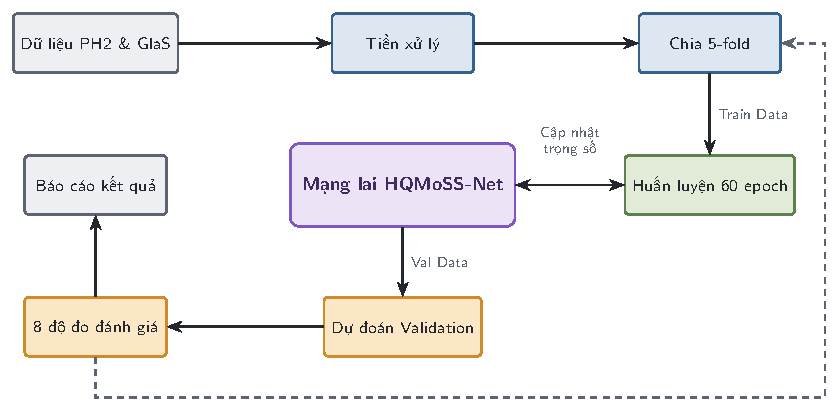
\includegraphics[width=\linewidth,height=0.66\textheight,keepaspectratio]{figures/fig_experiment_pipeline.pdf}
  \end{columns}
\end{frame}

% ---------- 10. KẾT QUẢ SO SÁNH ----------
\begin{frame}{Kết quả: so sánh với baseline}
  \begin{columns}[T]
    \column{0.48\textwidth}
      \centering\footnotesize
      \begin{tabular}{@{}lcc@{}}
        \toprule
        \textbf{Mô hình} & \textbf{Tham số} & \textbf{Soft IoU} \\
        \midrule
        U-Net            & 88K   & 0.779 \\
        UNet++           & 638K  & 0.793 \\
        Attention U-Net  & 644K  & 0.792 \\
        R2U-Net          & 1.87M & 0.806 \\
        QuNet (QuFeX)    & 84K   & 0.794 \\
        \midrule
        \textbf{HQMoSS-Net} & \textbf{154K} & \acc{0.850} \\
        \bottomrule
      \end{tabular}\\[0.3em]
      {\scriptsize Tập PH2 (trung bình 5-fold).}
    \column{0.52\textwidth}
      \centering
      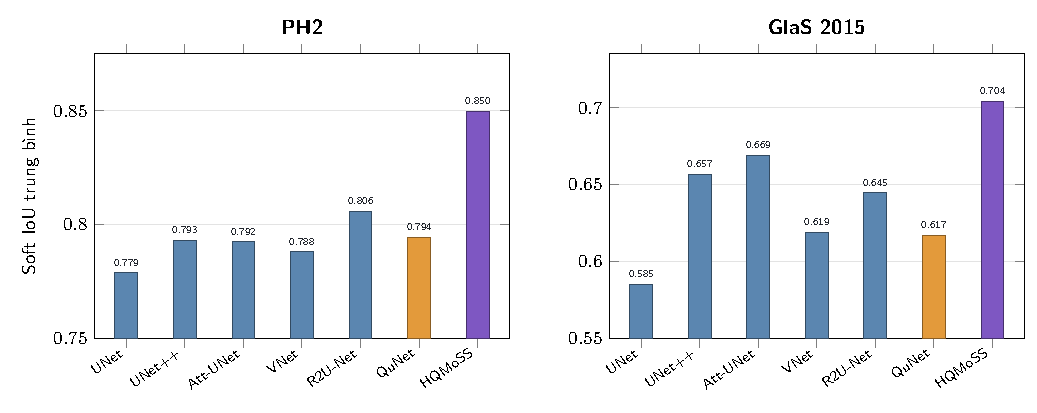
\includegraphics[width=\linewidth,height=0.62\textheight,keepaspectratio]{figures/fig_bar_models.pdf}
  \end{columns}
  \vspace{0.2em}
  {\footnotesize PH2: \hl{+7.1} điểm so với U-Net; GlaS: \hl{+11.9} điểm -- khoảng cách nới rộng trên tập khó hơn, đồng thời \acc{độ lệch chuẩn nhỏ hơn} (ổn định qua các fold).\par}
\end{frame}

% ---------- 11. HIỆU QUẢ THAM SỐ ----------
\begin{frame}{Hiệu quả tham số}
  \centering
  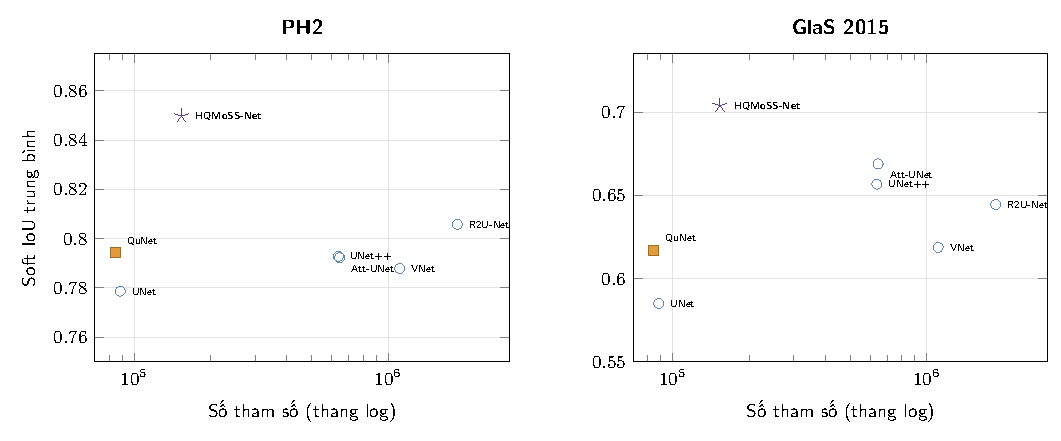
\includegraphics[width=0.86\linewidth,height=0.64\textheight,keepaspectratio]{figures/fig_scatter_efficiency.pdf}\\[0.4em]
  \small HQMoSS-Net (\acc{ngôi sao}) ở góc \hl{trên-trái}: IoU cao nhất trong khi số tham số thuộc nhóm thấp nhất -- vượt cả các baseline lớn hơn $4$--$12$ lần.
\end{frame}

% ---------- 12. BÓC TÁCH + CMOE ----------
\begin{frame}{Bóc tách thành phần \& đối chứng cổ điển}
  \begin{columns}[T]
    \column{0.56\textwidth}
      \centering
      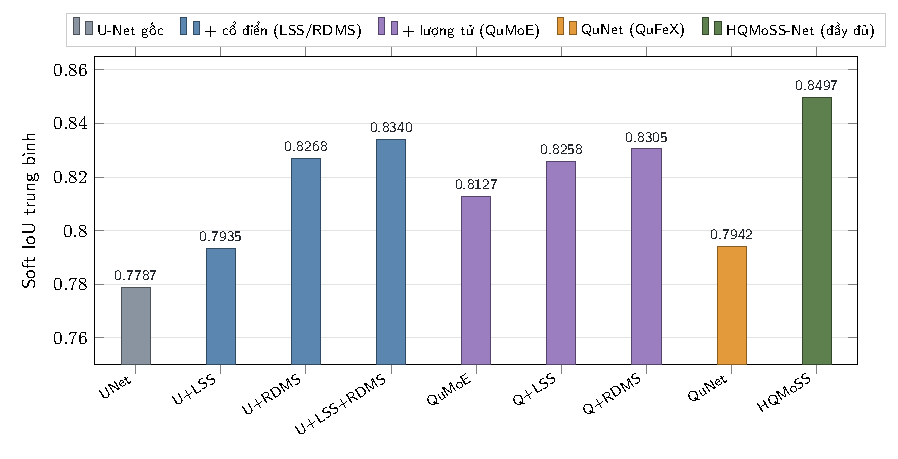
\includegraphics[width=\linewidth,height=0.58\textheight,keepaspectratio]{figures/fig_bar_components.pdf}\\
      {\scriptsize Đóng góp cộng dồn của LSS, RDMS, QuMoE (PH2).}
    \column{0.44\textwidth}
      \begin{itemize}
        \item Ba thành phần bổ trợ lẫn nhau: khi kết hợp cả ba, Soft IoU tăng \acc{+9.12\%} so với U-Net gốc.
        \item RDMS đóng góp lớn nhất ($+6.18\%$); QuMoE $+4.37\%$.
      \end{itemize}
      \begin{block}{QuantumMoE vs.\ Classical MoE (cùng kiến trúc)}
        \footnotesize Riêng tại khối bottleneck, CMoE có \acc{$1.609.763$} tham số, gấp khoảng \acc{$565$ lần} so với \acc{$2.851$} tham số của QuantumMoE. Tuy nhiên, tính trên toàn mô hình, mức chênh lệch này chỉ còn khoảng \acc{$19{,}5$ lần}. Dù vậy CMoE cho Soft IoU \emph{thấp hơn} (0.760 vs 0.813) và kém ổn định ($\pm0.14$ vs $\pm0.008$).
      \end{block}
  \end{columns}
\end{frame}

% ---------- 13. KIỂM ĐỊNH THỐNG KÊ ----------
\begin{frame}{Kiểm định ý nghĩa thống kê}
  \small Đơn vị: Soft IoU pooled mức fold ($K{=}5$). Bằng chứng chính: \hl{khoảng tin cậy bootstrap 95\%} (loại trừ 0 $=$ có ý nghĩa); kèm Cohen's d và $p$ một phía; gộp hai bộ dữ liệu bằng \hl{Stouffer's Z}.
  \vspace{0.3em}
  \begin{center}\footnotesize
  \renewcommand{\arraystretch}{1.25}
  \begin{tabular}{@{}lcc@{}}
    \toprule
    \textbf{Baseline} & \textbf{$\Delta_{\mathrm{PH2}}$ / $\Delta_{\mathrm{GlaS}}$ (\%)} & \textbf{$p$ gộp (Stouffer)} \\
    \midrule
    QuNet (QuFeX)   & 5.55 / 8.68  & $3.3\times10^{-5}$ \\
    R2U-Net         & 4.39 / 5.93  & 0.0007 \\
    V-Net (2D)      & 6.19 / 8.51  & 0.0011 \\
    U-Net           & 7.10 / 11.87 & 0.0022 \\
    Attention U-Net & 5.75 / 3.49  & 0.0115 \\
    UNet++          & 5.69 / 4.72  & 0.0179 \\
    \bottomrule
  \end{tabular}
  \end{center}
  {\footnotesize Trên PH2, cả sáu baseline có CI loại trừ 0. Gộp PH2+GlaS: \acc{$p<0.05$ với toàn bộ baseline} -- ưu thế đạt ý nghĩa thống kê rõ ràng.\par}
\end{frame}

% ---------- 15. XAI ĐỊNH LƯỢNG ----------
\begin{frame}{Khả giải thích (XAI) -- Seg-Grad-CAM: định lượng}
  \begin{itemize}
    \item Seg-Grad-CAM sinh bản đồ nhiệt vùng mô hình ``chú ý''; đo bằng tám chỉ số: IoU/Dice (Otsu \& matched), Boundary IoU, HD95, \hl{Energy Pointing Game}, Deletion/Insertion AUC.
    \item HQMoSS-Net \acc{tốt hơn U-Net trên hầu hết chỉ số} ở cả hai bộ dữ liệu (ví dụ Energy PG trên PH2: \acc{0.986} vs 0.958).
  \end{itemize}
  \vspace{0.2em}
  \centering
  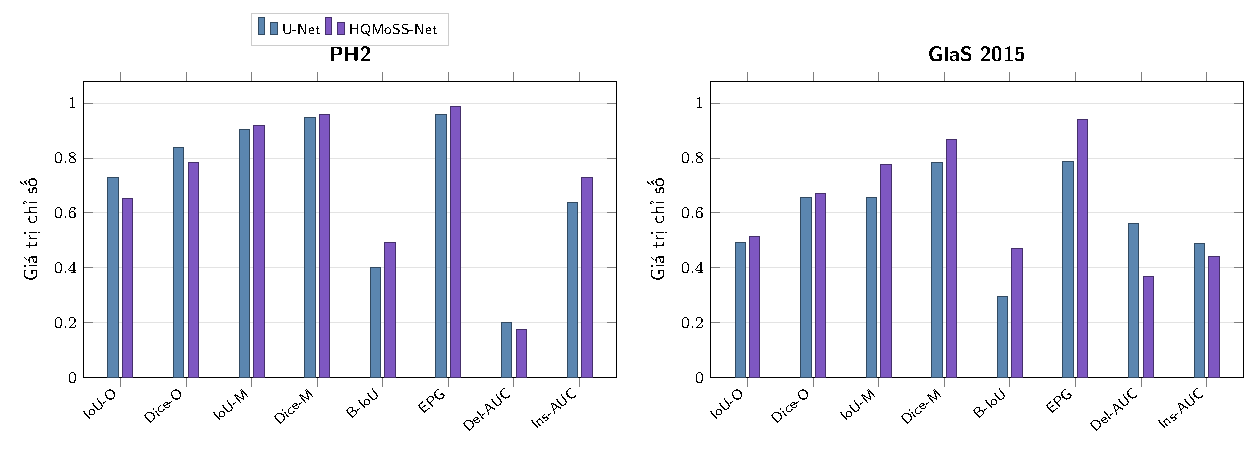
\includegraphics[width=0.98\linewidth,height=0.56\textheight,keepaspectratio]{figures/fig_xai_bar_metrics.pdf}\\
  {\scriptsize Tám chỉ số diễn giải (thang $[0,1]$) -- U-Net (xanh) vs HQMoSS-Net (tím): PH2 (trái), GlaS 2015 (phải).}
\end{frame}

% ---------- 16. XAI ĐỊNH TÍNH + HD95 ----------
\begin{frame}{Khả giải thích (XAI): định tính \& HD95}
  \begin{columns}[T]
    \column{0.64\textwidth}
      \centering
      {\scriptsize\hl{PH2} (tổn thương da)}\\[0.1em]
      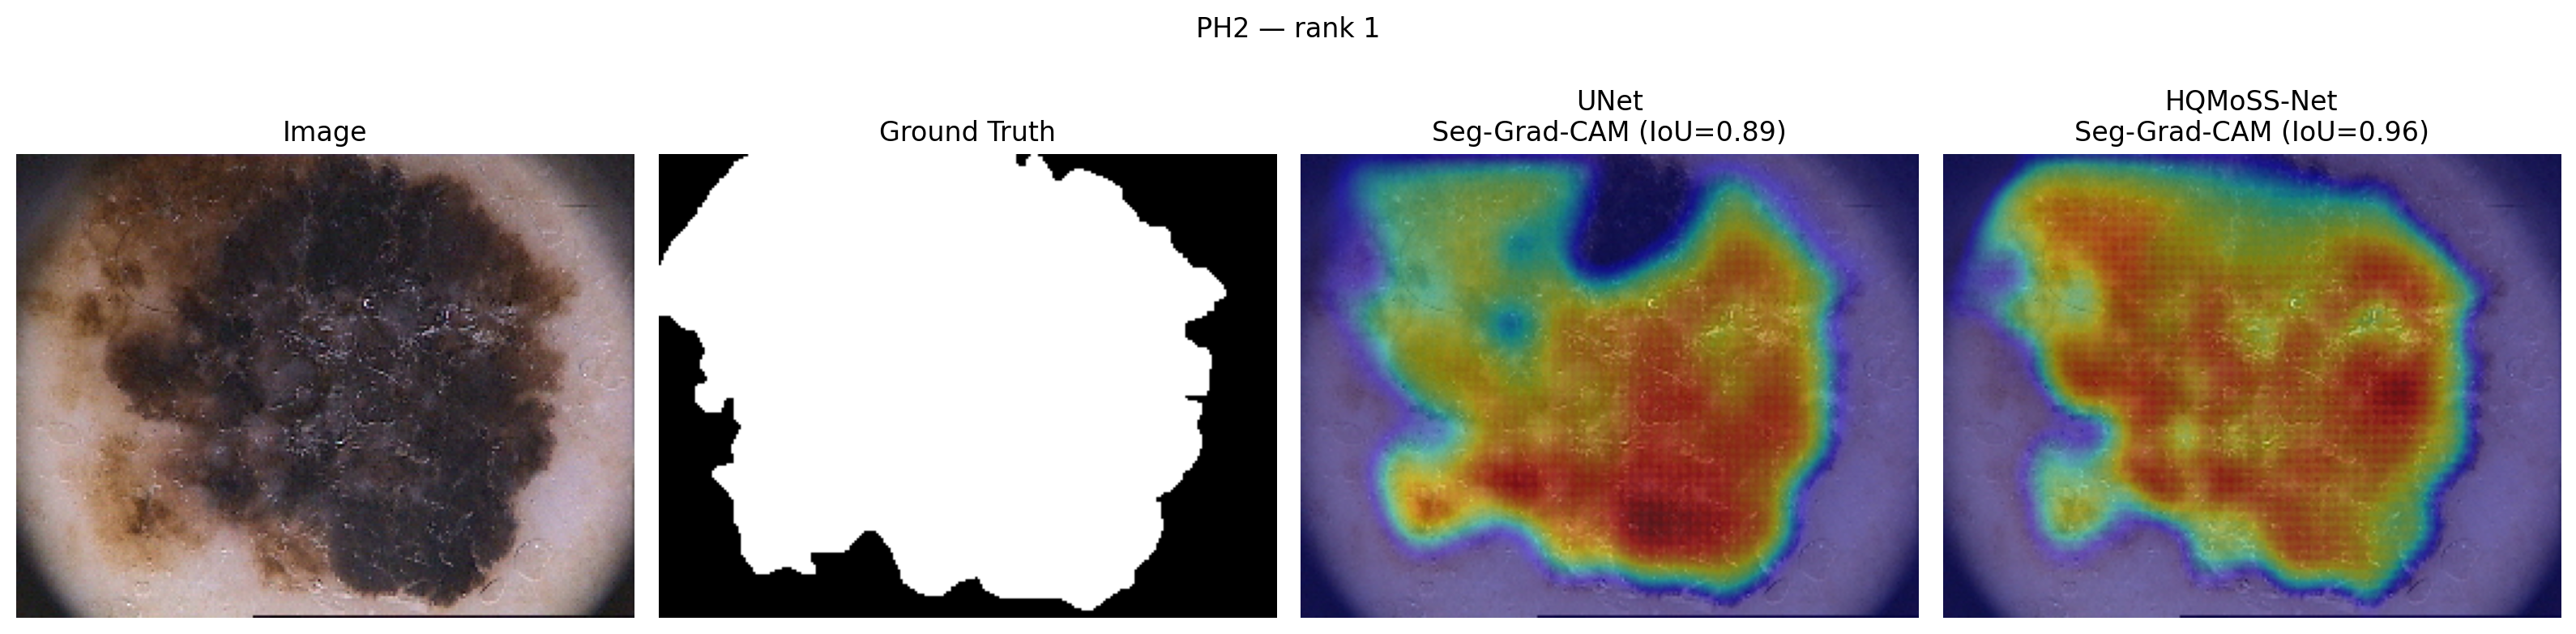
\includegraphics[width=\linewidth,height=0.27\textheight,keepaspectratio]{images/xai_cmp_ph2_1.png}\\[0.35em]
      {\scriptsize\hl{GlaS 2015} (mô học nhiều tuyến)}\\[0.1em]
      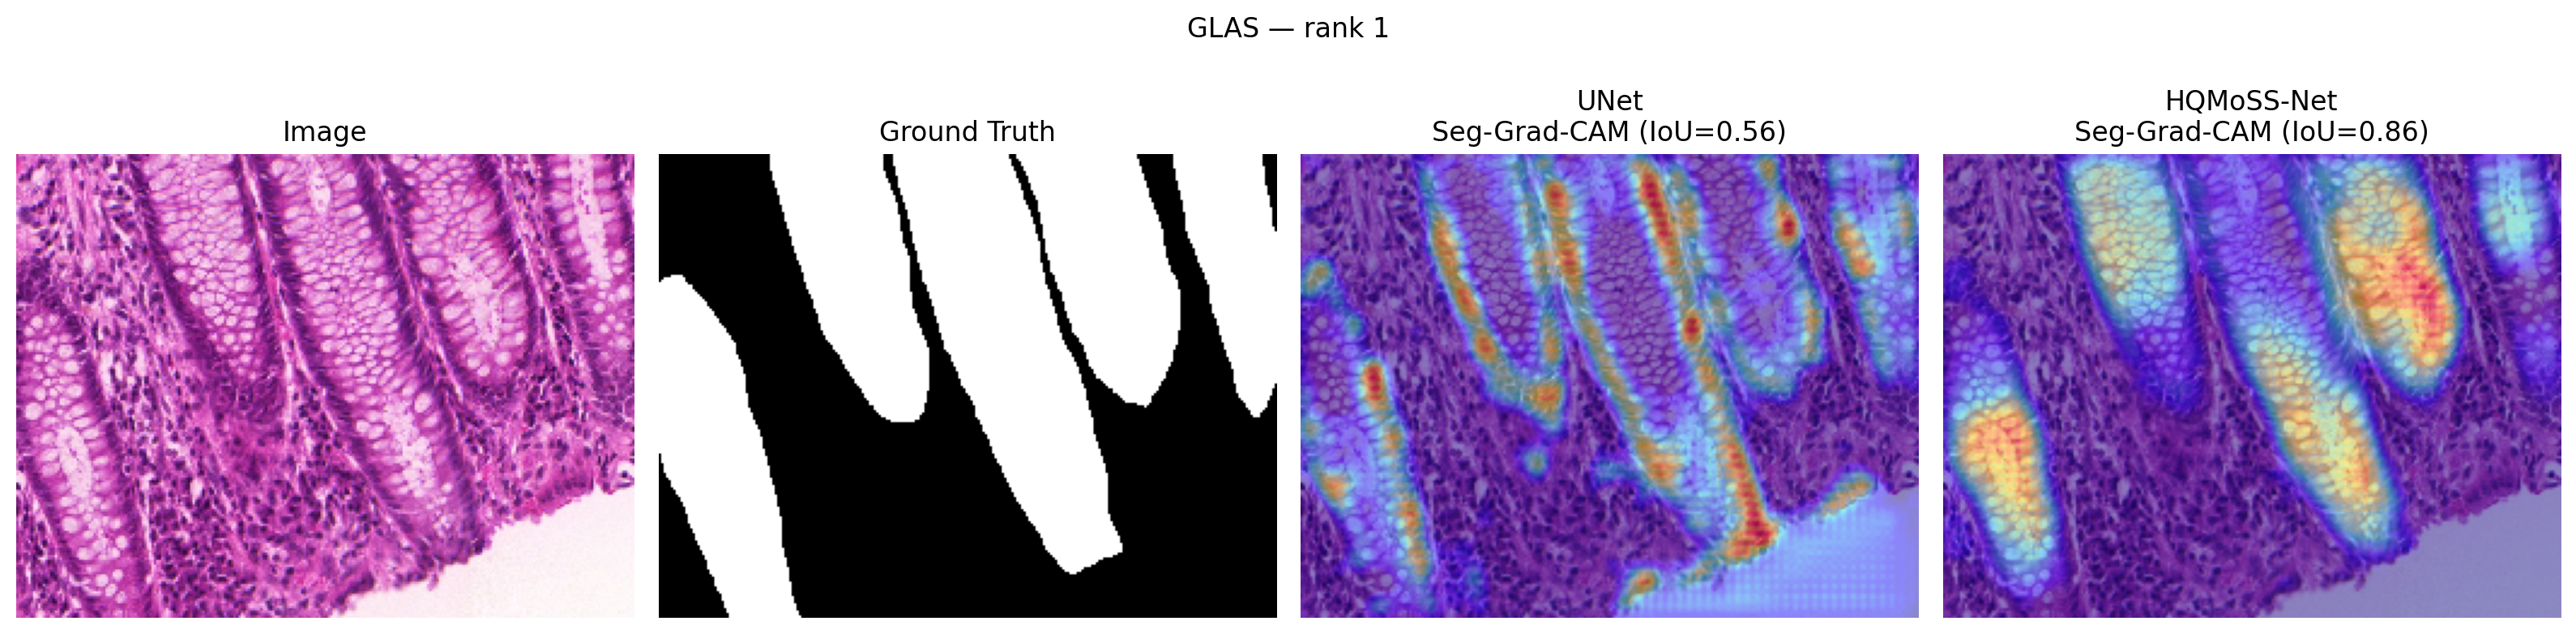
\includegraphics[width=\linewidth,height=0.27\textheight,keepaspectratio]{images/xai_cmp_glas_1.png}
    \column{0.36\textwidth}
      \centering
      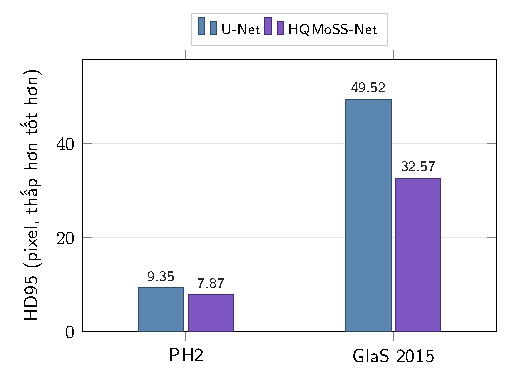
\includegraphics[width=\linewidth,height=0.5\textheight,keepaspectratio]{figures/fig_xai_hd95.pdf}\\[0.2em]
      {\scriptsize \hl{HD95} (đơn vị pixel, \acc{thấp hơn tốt hơn}): HQMoSS-Net thấp hơn U-Net trên cả hai bộ dữ liệu.}
  \end{columns}
  \vspace{0.3em}
  {\scriptsize\centering Mỗi hàng: ảnh gốc -- mặt nạ thực -- CAM U-Net -- CAM HQMoSS-Net (kèm IoU). Mô hình lai \acc{bám sát vùng đối tượng} hơn hẳn U-Net.\par}
\end{frame}

% ---------- 15. THẢO LUẬN / HẠN CHẾ ----------
\begin{frame}{Thảo luận \& hạn chế}
  \textbf{Điểm mạnh:}
  \begin{itemize}
    \item Cho kết quả tốt hơn mọi baseline trên cả hai bộ dữ liệu, với \hl{hiệu quả tham số} cao và ổn định.
    \item Đối chứng cổ điển và kiểm định thống kê cho thấy \hl{biểu diễn lượng tử} có đóng góp thực sự, dù mức cải thiện còn khiêm tốn.
  \end{itemize}
  \textbf{Hạn chế (nêu trung thực):}
  \begin{itemize}
    \item \acc{Chi phí mô phỏng} giả lập lượng tử cao, dẫn đến thời gian huấn luyện dài.
    \item Mới đánh giá trên \acc{hai bộ dữ liệu}; trên GlaS, ưu thế so với một vài baseline mạnh chưa đạt ý nghĩa thống kê rõ ràng, do số fold còn hạn chế ($K{=}5$).
    \item Đối chứng với Classical MoE mới dừng ở \acc{một cấu hình duy nhất}, chưa quét các biện pháp giảm quá khớp cho phía cổ điển nên chưa thể kết luận chắc chắn.
  \end{itemize}
\end{frame}

% ---------- 16. KẾT LUẬN ----------
\begin{frame}{Kết luận}
  \begin{block}{Đóng góp đã đạt}
    \begin{itemize}
      \item Đề xuất \hl{HQMoSS-Net}: nhúng QuantumMoE đa tỷ lệ + LSS tại nút thắt cổ chai của U-Net, kèm khối RDMS cổ điển.
      \item \hl{Nhỉnh hơn rõ rệt} so với các baseline cổ điển và lượng tử trên PH2 và GlaS, chỉ với 154K tham số.
      \item \hl{Quy trình đánh giá đầy đủ}: bóc tách, kiểm định thống kê, và khả giải thích Seg-Grad-CAM.
    \end{itemize}
  \end{block}
  \centering\small Ba thành phần đa tỷ lệ (cổ điển + lượng tử) và khối chuỗi tạo \acc{hiệu ứng cộng hưởng} đúng như giả thuyết thiết kế.
\end{frame}

% ---------- 17. HƯỚNG PHÁT TRIỂN + CẢM ƠN ----------
\begin{frame}{Hướng phát triển \& lời cảm ơn}
  \textbf{Hướng phát triển:}
  \begin{itemize}
    \item Thử nghiệm trên \hl{phần cứng lượng tử thực} (IBM Q, IonQ) kèm giảm nhiễu.
    \item Mở rộng \hl{đa lớp / ảnh 3D}; định tuyến thưa (top-$k$) giảm chi phí mô phỏng.
    \item Đối chứng cổ điển toàn diện hơn; mở rộng số bộ dữ liệu.
  \end{itemize}
  \vfill
  \begin{center}
    {\color{hcmusblue}\rule{0.7\textwidth}{1pt}}\\[0.6em]
    {\LARGE\bfseries\color{hcmusblue} Xin cảm ơn Hội đồng đã lắng nghe!}\\[0.4em]
    {\large Kính mời Hội đồng đặt câu hỏi.}\\[0.5em]
    {\color{hcmusblue}\rule{0.7\textwidth}{1pt}}
  \end{center}
\end{frame}

% ---------- 20. TÀI LIỆU THAM KHẢO CỐT LÕI ----------
\begin{frame}{Tài liệu tham khảo cốt lõi}
  \scriptsize
  \begin{enumerate}\setlength{\itemsep}{0.25em}
    \item N. Jain, A. Kalev. \textbf{QuFeX}: Quantum Feature Extraction Module for Hybrid Quantum-Classical Deep Neural Networks. \textit{Quantum Sci.\ Technol.}, 2026.
    \item H.-Q. Nguyen \emph{et al.} \textbf{QMoE}: A Quantum Mixture of Experts Framework for Scalable Quantum Neural Networks. \textit{arXiv:2507.05190}, 2025.
    \item M. Cerezo \emph{et al.} Variational Quantum Algorithms. \textit{Nature Reviews Physics}, 2021.
    \item A. Gu, T. Dao. \textbf{Mamba}: Linear-Time Sequence Modeling with Selective State Spaces. \textit{arXiv:2312.00752}, 2023.
    \item O. Ronneberger, P. Fischer, T. Brox. \textbf{U-Net}: Convolutional Networks for Biomedical Image Segmentation. \textit{MICCAI}, 2015.
    \item R. R. Selvaraju \emph{et al.} \textbf{Grad-CAM}: Visual Explanations from Deep Networks via Gradient-Based Localization. \textit{ICCV}, 2017.
    \item K. Vinogradova, A. Dibrov, G. Myers. \textbf{Seg-Grad-CAM}: Towards Interpretable Semantic Segmentation. \textit{AAAI}, 2020.
    \item T. Mendonça \emph{et al.} \textbf{PH2} -- A Dermoscopic Image Database. \textit{IEEE EMBC}, 2013.
    \item K. Sirinukunwattana \emph{et al.} Gland Segmentation in Colon Histology Images: The \textbf{GlaS} Challenge. \textit{Medical Image Analysis}, 2017.
  \end{enumerate}
  \vspace{0.6em}
  {\scriptsize\itshape Danh mục đầy đủ được trình bày trong cuốn báo cáo khóa luận.}
\end{frame}

% ================= PHỤ LỤC (backup cho hỏi đáp) =================
\appendix

% ---------- PHỤ LỤC A: huấn luyện mạch lượng tử ----------
\begin{frame}{Phụ lục A -- Khả năng huấn luyện mạch lượng tử}
  \begin{columns}[T]
    \column{0.52\textwidth}
      \textbf{Quy tắc dịch tham số (parameter-shift):}\\
      Gradient kỳ vọng lượng tử tính \hl{chính xác} bằng hai lần chạy mạch:
      {\footnotesize\[ \frac{\partial \langle O\rangle}{\partial\theta}=\tfrac{1}{2}\big[f(\theta{+}\tfrac{\pi}{2})-f(\theta{-}\tfrac{\pi}{2})\big] \]}
      $\Rightarrow$ mạch khả vi, huấn luyện đầu-cuối cùng phần cổ điển.
      \vspace{0.4em}

      \textbf{Cao nguyên cằn cỗi (barren plateau):}\\
      {\footnotesize Gradient triệt tiêu theo hàm mũ khi mạch quá sâu/rộng. Giảm thiểu: \hl{số qubit nhỏ} ($n\le9$), \hl{số lớp vừa} ($L\le5$), ansatz có cấu trúc $+$ kết nối phần dư.\par}
    \column{0.48\textwidth}
      \centering \textbf{\small Ablation số lớp mạch (PH2)}\\[0.2em]
      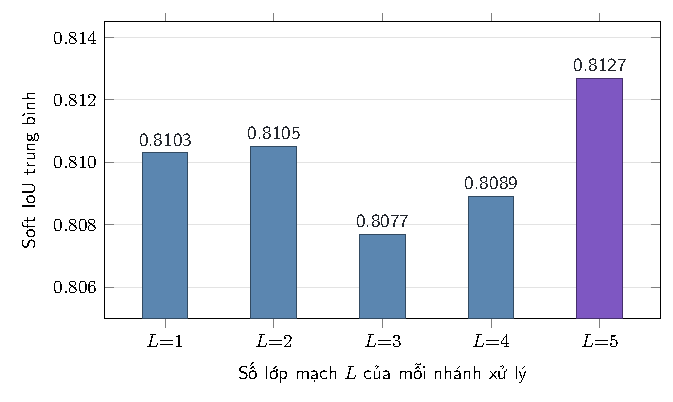
\includegraphics[width=\linewidth,height=0.44\textheight,keepaspectratio]{figures/fig_bar_layers.pdf}\\[0.2em]
      {\scriptsize $L{=}1\to5$: hiệu năng ổn định, tốt nhất tại $L{=}5$; độ lệch chuẩn \acc{giảm} ($\pm0.027\to\pm0.008$) $\Rightarrow$ chưa thấy dấu hiệu barren plateau.}
  \end{columns}
\end{frame}

% ---------- PHỤ LỤC B: cân bằng định tuyến ----------
\begin{frame}{Phụ lục B -- Phân tích cân bằng định tuyến (Router)}
  \begin{columns}[T]
    \column{0.5\textwidth}
      \small Kiểm chứng thiết kế: đưa \hl{đặc trưng gốc $F$} vào router giúp tránh \hl{sụp đổ nhánh xử lý} (Expert Collapse).
      \begin{itemize}
        \item Entropy định tuyến $>88\%$ mức tối đa -- \acc{không nhánh nào bị bỏ trống}.
        \item PH2: CV $0.27$ (thiên nhánh cục bộ); GlaS: CV $0.09$ (cân bằng hơn, huy động nhánh toàn cục).
        \item Kiểm định Mann-Whitney U: phân bổ khác nhau \acc{có ý nghĩa} giữa hai bộ $\Rightarrow$ router \hl{thích nghi theo đặc tính dữ liệu}.
      \end{itemize}
      {\scriptsize\itshape (Phân tích trên một checkpoint đại diện -- fold 1.)}
    \column{0.5\textwidth}
      \centering
      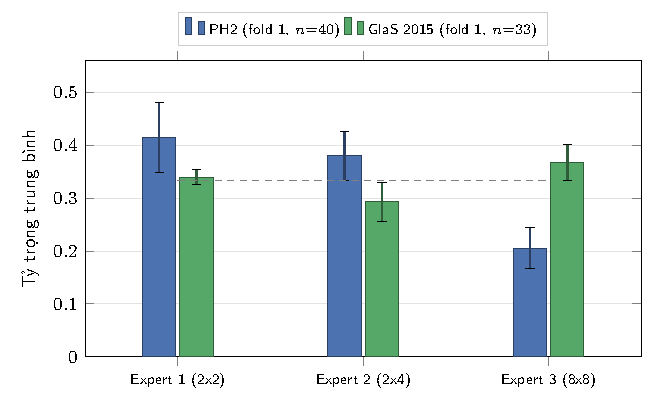
\includegraphics[width=\linewidth,height=0.66\textheight,keepaspectratio]{figures/fig_router_balance.pdf}
  \end{columns}
\end{frame}

% ---------- PHỤ LỤC C: độ đo XAI & lập luận thiết kế ----------
\begin{frame}{Phụ lục C -- Độ đo XAI \& lập luận thiết kế}
  \begin{columns}[T]
    \column{0.5\textwidth}
      \textbf{\small Tám độ đo diễn giải (3 nhóm):}
      \begin{itemize}\footnotesize
        \item \hl{Định vị} -- mức chồng lấp CAM với vùng thực:
          \begin{itemize}\scriptsize
            \item \emph{IoU/Dice (Otsu \& matched)}: nhị phân hóa CAM (ngưỡng Otsu / khớp diện tích) rồi so với ground-truth.
            \item \emph{Energy Pointing Game}: \% ``năng lượng'' CAM rơi trong vùng thực (không cần ngưỡng).
          \end{itemize}
        \item \hl{Đường biên} -- độ khớp đường viền:
          \begin{itemize}\scriptsize
            \item \emph{Boundary IoU}: IoU tính riêng trên dải biên.
            \item \emph{HD95}: khoảng cách biên (phân vị 95; thấp hơn tốt hơn).
          \end{itemize}
        \item \hl{Trung thực} -- CAM có phản ánh đúng pixel chi phối:
          \begin{itemize}\scriptsize
            \item \emph{Deletion/Insertion AUC}: xóa/chèn dần pixel theo CAM, đo dự đoán sụp/phục hồi.
          \end{itemize}
      \end{itemize}
    \column{0.5\textwidth}
      \centering\scriptsize \textbf{Lập luận thiết kế $\to$ kết quả}\\[0.2em]
      \renewcommand{\arraystretch}{1.2}
      \begin{tabular}{@{}>{\raggedright\arraybackslash}p{2.4cm}>{\raggedright\arraybackslash}p{4.0cm}@{}}
        \toprule
        \textbf{Lựa chọn} & \textbf{Kết quả quan sát} \\
        \midrule
        Bộ khung U-Net & Bảo toàn không gian; nền tảng vững \\
        RDMS đa tỷ lệ & $+6.18\%$ (thành phần cổ điển lớn nhất) \\
        QuantumMoE & $+4.37\%$; cộng hưởng RDMS $+6.65\%$ \\
        LSS & Đẩy cấu hình đầy đủ lên $+9.12\%$ \\
        Router có $F$ & Định tuyến cân bằng, không sụp đổ \\
        \bottomrule
      \end{tabular}
  \end{columns}
\end{frame}

\end{document}
